% Graphic for TeX using PGF
% Title: /home/FatLord/Diagrama3.dia
% Creator: Dia v0.97.3
% CreationDate: Wed Oct  7 22:16:45 2015
% For: FatLord
% \usepackage{tikz}
% The following commands are not supported in PSTricks at present
% We define them conditionally, so when they are implemented,
% this pgf file will use them.
\ifx\du\undefined
  \newlength{\du}
\fi
\setlength{\du}{15\unitlength}
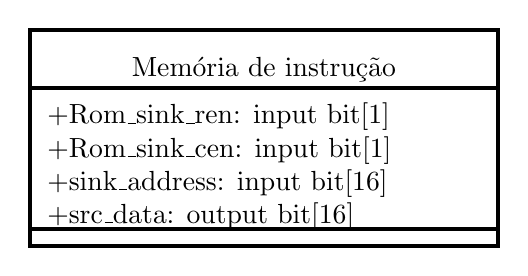
\begin{tikzpicture}
\pgftransformxscale{1.000000}
\pgftransformyscale{-1.000000}
\definecolor{dialinecolor}{rgb}{0.000000, 0.000000, 0.000000}
\pgfsetstrokecolor{dialinecolor}
\definecolor{dialinecolor}{rgb}{1.000000, 1.000000, 1.000000}
\pgfsetfillcolor{dialinecolor}
\pgfsetlinewidth{0.100000\du}
\pgfsetdash{}{0pt}
\definecolor{dialinecolor}{rgb}{1.000000, 1.000000, 1.000000}
\pgfsetfillcolor{dialinecolor}
\fill (20.450000\du,7.300000\du)--(20.450000\du,8.700000\du)--(31.730000\du,8.700000\du)--(31.730000\du,7.300000\du)--cycle;
\definecolor{dialinecolor}{rgb}{0.000000, 0.000000, 0.000000}
\pgfsetstrokecolor{dialinecolor}
\draw (20.450000\du,7.300000\du)--(20.450000\du,8.700000\du)--(31.730000\du,8.700000\du)--(31.730000\du,7.300000\du)--cycle;
% setfont left to latex
\definecolor{dialinecolor}{rgb}{0.000000, 0.000000, 0.000000}
\pgfsetstrokecolor{dialinecolor}
\node at (26.090000\du,8.250000\du){Memória de instrução};
\definecolor{dialinecolor}{rgb}{1.000000, 1.000000, 1.000000}
\pgfsetfillcolor{dialinecolor}
\fill (20.450000\du,8.700000\du)--(20.450000\du,12.100000\du)--(31.730000\du,12.100000\du)--(31.730000\du,8.700000\du)--cycle;
\definecolor{dialinecolor}{rgb}{0.000000, 0.000000, 0.000000}
\pgfsetstrokecolor{dialinecolor}
\draw (20.450000\du,8.700000\du)--(20.450000\du,12.100000\du)--(31.730000\du,12.100000\du)--(31.730000\du,8.700000\du)--cycle;
% setfont left to latex
\definecolor{dialinecolor}{rgb}{0.000000, 0.000000, 0.000000}
\pgfsetstrokecolor{dialinecolor}
\node[anchor=west] at (20.600000\du,9.400000\du){+Rom\_sink\_ren: input bit\ensuremath{[}1\ensuremath{]}};
% setfont left to latex
\definecolor{dialinecolor}{rgb}{0.000000, 0.000000, 0.000000}
\pgfsetstrokecolor{dialinecolor}
\node[anchor=west] at (20.600000\du,10.200000\du){+Rom\_sink\_cen: input bit\ensuremath{[}1\ensuremath{]}};
% setfont left to latex
\definecolor{dialinecolor}{rgb}{0.000000, 0.000000, 0.000000}
\pgfsetstrokecolor{dialinecolor}
\node[anchor=west] at (20.600000\du,11.000000\du){+sink\_address: input bit\ensuremath{[}16\ensuremath{]}};
% setfont left to latex
\definecolor{dialinecolor}{rgb}{0.000000, 0.000000, 0.000000}
\pgfsetstrokecolor{dialinecolor}
\node[anchor=west] at (20.600000\du,11.800000\du){+src\_data: output bit\ensuremath{[}16\ensuremath{]}};
\definecolor{dialinecolor}{rgb}{1.000000, 1.000000, 1.000000}
\pgfsetfillcolor{dialinecolor}
\fill (20.450000\du,12.100000\du)--(20.450000\du,12.500000\du)--(31.730000\du,12.500000\du)--(31.730000\du,12.100000\du)--cycle;
\definecolor{dialinecolor}{rgb}{0.000000, 0.000000, 0.000000}
\pgfsetstrokecolor{dialinecolor}
\draw (20.450000\du,12.100000\du)--(20.450000\du,12.500000\du)--(31.730000\du,12.500000\du)--(31.730000\du,12.100000\du)--cycle;
\end{tikzpicture}
